\documentclass[lang=cn,newtx,10pt,scheme=chinese]{elegantbook}

% 简称
\newcommand{\wf}{WolfRAM}
\newcommand{\dr}{???}
\newcommand{\wkn}{WeiKnight}

\title{\wkn{}设定与世界观公式书}
\subtitle{基于理论模型的设定公式书}

\author{\wkn{}}
% \institute{Elegant\LaTeX{} Program}
\date{2025}
% \version{4.5}
% \bioinfo{自定义}{信息}

\extrainfo{注意:本公式书仅供娱乐}

\setcounter{tocdepth}{3}

\logo{logo.png}
\cover{cover.jpg}

% 本文档命令
\usepackage{array}
\newcommand{\ccr}[1]{\makecell{{\color{#1}\rule{1cm}{1cm}}}}

% 修改标题页的橙色带
\definecolor{customcolor}{RGB}{32,178,170}
\colorlet{coverlinecolor}{customcolor}
\usepackage{cprotect}
\usepackage{mathtools}
\usepackage{physics}
\usepackage{float}
\usepackage{xcolor}

% \addbibresource[location=local]{reference.bib} % 参考文献,不要删除

\newcommand{\md}{\mathrm{d}}
\newcommand{\me}{\mathrm{e}}
\newcommand{\mj}{\mathrm{j}}


% 神理论
\newcommand{\dom}{\mathop{\mathrm{dom}}} % 掌控域
\newcommand{\Divine}{\mathcal{D}} % 神性谓词
\newcommand{\G}{\mathfrak{G}} % 神符号
\DeclareMathOperator{\Controls}{Controls} % 掌控关系

\begin{document}

\maketitle
\frontmatter

\tableofcontents

\mainmatter

\chapter*{文档说明}
\markboth{文档说明}{文档说明}
这个公式书基于Elegant \LaTeX{}编写。项目地址:\href{https://github.com/ElegantLaTeX/ElegantBook}{https://github.com/ElegantLaTeX/ElegantBook}

本书主要涵盖以下内容:
\begin{introduction}
    \item 世界观之上的基本规律的介绍
    \item 世界观的基本介绍
    \item \wkn{}的OC的介绍
\end{introduction}

本OC公式书中的设定图像、设定文字归\wkn{}或其画师所有,未经允许不得转载!

OC公式书的项目地址:\href{https://github.com/WeiKnight0/MySettingOC}{https://github.com/WeiKnight0/MySettingOC} 欢迎Star!

\chapter{世界观规律的基本介绍}
本章主要介绍OC所在的世界观的基本规律的介绍。涵盖以下内容:
\begin{introduction}
    \item 世界观的数学基础
    \item 世界观的计算机基础
    \item 实用函数与能力
    \item 世界理论与无神理论
    \item 元素理论
    \item 二次元变换
\end{introduction}

\section{世界观的数学基础}
这一节主要介绍世界观中可能用到的数学知识。
\begin{introduction}
    \item 矢量/向量
    \item 矩阵与高等代数
    \item 一元函数的微分与积分
    \item 平面解析几何
    \item 立体几何与空间解析几何
    \item 多元函数微分
    \item 二重积分与三重积分
    \item 曲线积分与曲面积分
    \item 概率统计知识
    \item 复变函数
    \item 常微分方程
\end{introduction}
具体知识请参考有关的数学教材。

\section{世界观的计算机基础}
这一节主要介绍世界观中可能用到的计算机知识。
\begin{introduction}
    \item 数字逻辑电路
    \item 数据结构与算法
    \item 类与对象
    \item 连续时间傅里叶变换与离散傅里叶变换
    \item 拉普拉斯变换与\(z\)变换
\end{introduction}
具体知识请参考有关的计算机教材。

\section{实用函数与能力}
这一节主要介绍实用函数理论和能力知识。
\begin{introduction}
    \item 函数与实用函数
    \item 能力系统
    \item 传参型实用函数
    \item 积分型实用函数
    \item 符咒
    \item 微分符咒
\end{introduction}

\subsection{函数与实用函数}
数学上定义\textbf{函数}是\textbf{从定义域到值域的一种对应关系},又称为\textbf{映射}。对于定义域中的每个元素,
均能在值域中找到对应的元素。此时称定义域中的元素为\textbf{原像},值域中的对应的元素为\textbf{像}。对于值域
而言,取其中每个
所有存在原像的元素组成子集,称为\textbf{陪域}。若值域等于陪域,则称这个函数为\textbf{满射函数}。

没有特别说明,之后涉及的所有函数均为满射函数。

在二次元世界,常常有各种能力,这些能力作用于二次元的物体,使之发生变化,相当于产生了一个映射。我们可以将这样的
映射近似地看作数学函数。此时的函数被称作\textbf{实用函数}。

实用函数有以下特点:

% \begin{minipage}[b]{0.9\textwidth}
\begin{enumerate}
    \item \textbf{定义域未必是数的集合。}实用函数的定义域可能只是一个角色,一个物体,甚至可以是某个
          抽象的二次元中的概念。只要符合实用函数的定义均为实用函数。
    \item \textbf{值域未必是数的集合。}与定义域类似,值域也可以不是数的集合。
    \item \textbf{通过角色的能力体现。}不同于数学函数,实用函数一般是角色能力的抽象,可能无法通过计算体现。
\end{enumerate}
% \end{minipage}

\subsection{能力系统}
\textbf{系统}是一系列成分组成的有机整体,而\textbf{能力系统}则是\textbf{运用角色能力的过程体现}。它
通过使用角色的能力,将某个二次元概念由某种状态转向另一种状态。例如,攻击能力系统将角色的HP由更高的HP转向
更低的HP。

\textbf{能力系统是实用函数的载体。}世界观中能力系统的存在保证了世界的正常运行。

\subsection{传参型实用函数}
根据实用函数的作用方式的不同,可以将实用函数分为\textbf{传参型实用函数}与\textbf{积分型实用函数}。传参型实用函数将
作用对象当作参数传入函数;积分型实用函数则是将作用对象当作积分域进行积分。

\begin{definition}[传参型实用函数]
    形为
    \[
        y = F(x)
    \]
    的实用函数\(F(x)\)是\textbf{传参型实用函数}。其中$x$为作用对象,$y$为作用结果。
\end{definition}

\begin{example}[治愈能力]
    设角色A拥有治愈能力,可以恢复目标50点HP。这可以表示为:
    \[
        \text{HP}' = \text{Heal}(\text{HP}) = \text{HP} + 50
    \]
    其中$\text{Heal}$是传参型实用函数。
\end{example}

\subsection{积分型实用函数}

\begin{definition}[积分型实用函数]
    实用函数\(f(x)\)的作用方式为
    \[
        y = \int_S f(x)\, \md x
    \]
    的函数是\textbf{积分型实用函数}。其中$S$为作用范围或\textbf{作用域},$y$为作用结果,
    \(x\)为\textbf{作用范围中的微元}。此时\(f(x)\)也称为\textbf{作用密度函数}。
\end{definition}

积分型实用函数与传参型实用函数的一个主要区别为,传参型实用函数的作用对象是一个整体,例如角色、物体;而积分型实用函数的作用对
象是一个连续的范围,例如空间、时间。

\begin{example}[范围伤害]
    角色B释放一个范围火球术,对区域$D$内所有敌人造成伤害。设火球术的伤害密度函数为$f(p)=100\me^{-|p|^2}$,
    则总伤害可表示为:
    \[
        \text{Damage} = \iint_D f(p)\, \md p
    \]
    这是一个典型的积分型实用函数。
\end{example}

\subsection{符咒}
\textbf{符咒}是世界观中一种特殊的\textbf{实用函数运算工具},对应于数学中的各种算子。符咒可以改变实用函数的作用方式或效果,是能力系统的重要组成部分。

\begin{definition}[符咒]
    符咒$\mathcal{O}$是一个作用于实用函数的映射:
    \[
        \mathcal{O}: F \mapsto \mathcal{O}F
    \]
    其中$F$是实用函数,$\mathcal{O}F$是经过符咒作用后的新实用函数。
\end{definition}

符咒具有以下特性:
\begin{enumerate}
    \item \textbf{线性性}:部分符咒满足线性性质,即
          \[
              \mathcal{O}(aF + bG) = a\mathcal{O}F + b\mathcal{O}G
          \]
    \item \textbf{复合性}:符咒可以组合使用,形成更复杂的符咒:
          \[
              (\mathcal{O}_1 \circ \mathcal{O}_2)F = \mathcal{O}_1(\mathcal{O}_2F)
          \]
    \item \textbf{特异性}:某些符咒只对特定类型的实用函数有效
\end{enumerate}

常见的符咒类型:
\begin{itemize}
    \item \textbf{时域冲激符咒} $\delta$:使实用函数产生瞬时作用效果
          \[
              \delta F(x) = F(x)\cdot \delta(0)
          \]
          其中\(\delta(t)\)是冲激函数。满足:
          \[
              \begin{dcases}
                  \delta(t) =0,\, t \neq 0                   \\
                  \int_{-\infty}^{+\infty}\delta(t)\,\md t=1 \\
              \end{dcases}
          \]
          % \item \textbf{微分符咒} $\nabla$:
    \item \textbf{时域积分符咒} $\mathcal{I}$:使实用函数产生"累积效果"
          \[
              \mathcal{I}F = \int_{-\infty}^t F\,\md \tau
          \]
    \item \textbf{强化符咒} $\mathcal{E}_k$:将实用函数效果放大$k$倍
          \[
              \mathcal{E}_k F = k \cdot F
          \]
\end{itemize}


符咒的合理组合与运用是世界观中角色能力开发的核心机制,高阶能力往往通过多重符咒的叠加与组合实现。

\subsection{微分符咒}

\textbf{微分符咒$\nabla$}是世界观中最为强大的空间变化符咒之一,对应于数学中的\textbf{梯度算子}。该符咒可以同时操控空间中的多种变化率,根据不同的组合方式实现高斯公式、格林公式等强大效果。

\subsubsection{微分符咒的概念}

\begin{definition}[微分符咒]
    在三维空间中,微分符咒$\nabla$定义为:
    \[
        \nabla = \left(\frac{\partial}{\partial x}, \frac{\partial}{\partial y}, \frac{\partial}{\partial z}\right)
    \]
    该符咒可以作用于标量场$\varphi$或向量场$\bm{F}=(F_x,F_y,F_z)$,产生不同效果:
    \begin{align*}
        \text{梯度符咒} & : \nabla\varphi = \left(\frac{\partial\varphi}{\partial x}, \frac{\partial\varphi}{\partial y}, \frac{\partial\varphi}{\partial z}\right)                                                                                                   \\
        \text{散度符咒} & : \nabla\cdot\bm{F} = \frac{\partial F_x}{\partial x} + \frac{\partial F_y}{\partial y} + \frac{\partial F_z}{\partial z}                                                                                                                   \\
        \text{旋度符咒} & : \nabla\times\bm{F} = \left(\frac{\partial F_z}{\partial y} - \frac{\partial F_y}{\partial z}, \frac{\partial F_x}{\partial z} - \frac{\partial F_z}{\partial x}, \frac{\partial F_y}{\partial x} - \frac{\partial F_x}{\partial y}\right)
    \end{align*}
\end{definition}

\subsubsection{微分符咒的应用}
微分符咒$\nabla$可以产生强大的效果。主要的效果就是\textbf{作用域的扩大}。

\begin{theorem}[高斯符咒公式]
    当$\nabla$符咒与闭合曲面积分$\oiint$组合时,可实现\textbf{作用域从曲面域到空间域的变化}:
    \[
        \oiint_{\partial V} \bm{F}\cdot\mathrm{d}\bm{S}=\iiint_V (\nabla\cdot\bm{F}) \,\md V
    \]
    此时作用范围扩大,由空间的包裹曲面域变化到了空间域。
\end{theorem}

\begin{example}[净化结界展开]
    角色A发动$\nabla\cdot$符咒检测体内邪气密度$\nabla\cdot\bm{D}$,然后通过高斯符咒公式将总邪气量转化为结界净化力:
    \[
        \text{净化力} = \oiint_{\partial \text{Body}} \bm{D}\cdot\mathrm{d}\bm{S}
    \]
\end{example}

\begin{theorem}[格林符咒公式]
    在二维平面上,$\nabla$符咒定义为:
    \[
        \nabla_{\text{2D}} = \left(\frac{\partial}{\partial x}, \frac{\partial}{\partial y}\right),\,
        \nabla_{\text{2D}}\times \bm{F}=\frac{\partial F_y}{\partial x} - \frac{\partial F_x}{\partial y}
    \]
    与闭合曲线积分$\oint$组合:
    \[
        \oint_C (L\mathrm{d}x + M\mathrm{d}y) = \iint_D \left(\frac{\partial M}{\partial x} - \frac{\partial L}{\partial y}\right) \mathrm{d}x\mathrm{d}y
    \]
    此时实现了作用域由曲线到曲线包围的平面的变化。
\end{theorem}

\begin{example}[风之领域]
    角色B创造风场$\bm{W} = (-y,x)$,使用格林符咒计算领域能量:
    \[
        \text{领域能量} = \oint_{\text{Circle}} \bm{W}\cdot\mathrm{d}\bm{r} = 2\iint_{D} \mathrm{d}A = 2\pi R^2
    \]
\end{example}

\begin{theorem}[斯托克斯符咒公式]
    对于空间曲线,$\nabla$符咒与闭合曲线积分$\oint$组合:
    \[
        \oint_C \bm{F}\cdot\mathrm{d}\bm{r} = \iint_S (\nabla\times\bm{F})\cdot\mathrm{d}\bm{S}
    \]
    此时作用范围由空间曲线转化为空间曲面。
\end{theorem}

\begin{example}[空间切割]
    角色C使用旋度符咒$\nabla\times$生成空间裂缝$\bm{V} = (0,-z,y)$,沿着圆形路径$C$实施切割:
    \[
        \text{切割强度} = \oint_C \bm{V}\cdot\mathrm{d}\bm{r} = \iint_{\text{Disk}} 2\mathrm{d}S = 2\pi R^2
    \]
\end{example}


\section{世界理论与无神理论}
这一节主要介绍世界理论与无神理论。
\begin{introduction}
    \item 世界与世界的性质
    \item 世界的层级关系
    \item 神与神的基本原理
    \item 无神定理
\end{introduction}

\subsection{世界与世界的性质}
在模态逻辑框架下,\textbf{一个世界是满足极大一致性的命题集
    合及其对应实体关系的完备
    结构,或等价地表述为可能状态空间中的极大连通分支}。根据
表述的不同,可以分为\textbf{世界的模态实在论}与\textbf{世界的代
    数拓扑表述}。

\begin{definition}[世界的模态实在论]
    一个世界 $w$ 是四元组 $(D_w, \varPhi_w, V_w, \prec_w)$ ,满足:
    \begin{enumerate}
        \item \textbf{域(Domain)}: $D_w \neq \emptyset$ 为该世界中的个体集合
        \item \textbf{命题空间}: $\varPhi_w$ 是$w$中所有命题的完备集,满足:
              \begin{itemize}
                  \item 封闭性: $\varphi \in \varPhi_w \Rightarrow \neg\varphi \in \varPhi_w$
                  \item 极大一致性: $\forall\varphi,\ \varphi \in \varPhi_w \oplus \neg\varphi \in \varPhi_w$
              \end{itemize}
        \item \textbf{赋值函数}: $V_w: \varPhi_w \to \{0,1\}$ 且 $V_w(\varphi) \neq V_w(\neg\varphi)$
        \item \textbf{可达关系}: $\prec_w \subseteq W \times W$ 表示可能世界关系。其中\(W\)表示所有可能世界的集合。
    \end{enumerate}
\end{definition}

\begin{definition}[世界的代数拓扑表述]
    在Stone空间$\mathcal{W}$上,世界是极大连通分支:
    \[ w \in \pi_0(\mathcal{W}, \tau) \]
    其中$\tau$为由基本命题生成的拓扑,$\pi_0$为连通分支函子。
\end{definition}

\begin{theorem}[世界的基本性质]
    \begin{enumerate}
        \item \textbf{存在性}: ZFC下存在基数$\kappa$使$|W| \geq 2^\kappa$
        \item \textbf{不可区分性}:
              $\forall \varphi \in \varPhi_{w_1} \cap \varPhi_{w_2},\, V_{w_1}(\varphi)=V_{w_2}(\varphi) \Rightarrow w_1 = w_2$
        \item \textbf{认知封闭性}: $\forall w,\ \exists\varphi_w,\ \forall w' \neq w,\ \varphi_w \notin \varPhi_{w'}$
    \end{enumerate}
\end{theorem}

\subsection{世界的层级关系}

\begin{definition}[可达关系]
    在可能世界集合$W$上,可达关系 $\prec \subseteq W \times W$ 满足:
    \begin{itemize}
        \item 非自反性:$\forall w \in W, w \nprec w$
        \item 命题扩张性:若$w_1 \prec w_2$,则$\varPhi_{w_1} \subsetneq \varPhi_{w_2}$
    \end{itemize}
\end{definition}

\begin{theorem}{世界的层级结构}{worldhierarchy}
    \begin{enumerate}
        \item \textbf{非对称真值赋值}:
              对于任意$w_1 \prec w_2$,存在真值函数$V_{w_i}$满足:
              \[
                  V_{w_1}(\lozenge \varphi_{w_2}) = 1 \quad \text{但} \quad V_{w_2}(\square \varphi_{w_1}) \text{未定义}
              \]
              其中$\lozenge$表示"可能",$\square$表示"必然"。

        \item \textbf{世界扩展性}:
              对任何$w \in W$,总存在$w' \in W$使得:
              \[
                  w \prec w' \quad \text{且} \quad |\varPhi_{w'}| > |\varPhi_w|
              \]

        \item \textbf{真值隔离}:
              若$w_1 \prec w_2$,则存在命题$\psi \in \varPhi_{w_2}$使得:
              \[
                  \psi \text{在} w_2 \text{中可判定,但在} w_1 \text{中无意义}
              \]
    \end{enumerate}
\end{theorem}

\begin{proof}[世界层次理论的哲学依据]
    % 该定理的形式化基于以下原则:
    \begin{itemize}
        \item \textbf{认知渐进性}:更“高阶”的世界包含更丰富的命题
        \item \textbf{真值相对性}:真值判断不能逆向传递
        \item \textbf{避免自指}:通过层级结构消除形如“本世界为假”的悖论
    \end{itemize}
\end{proof}

\begin{example}
    考虑三个世界组成的链:
    \[
        w_0 \prec w_1 \prec w_2
    \]
    \begin{itemize}
        \item 在$w_0$中:“$w_1$是可能的”为真,但无法谈论$w_2$
        \item 在$w_1$中:可以验证$w_0$的部分命题,但新增命题(如选择公理)在$w_0$中无意义
        \item $w_2$包含所有$w_0,w_1$的命题,并扩展了新的不可判定命题
    \end{itemize}
\end{example}

\subsection{神与神的基本原理}

在世界理论中,\textbf{神是存在某个主掌控世界及其所有子世界中的全能力智能体}
,能掌握
直接的一切,并对世界产生主观的任意影响。

\begin{definition}[神性智能体]
    一个神是四元组 $\G = (w_\G, \dom(\G), \Controls_\G, P_\G)$ 其中:
    \begin{itemize}
        \item $w_\G \in W$ 是主掌控世界
        \item $\dom(\G) \subseteq \mathrm{Cone}^-(w_\G)$ 是掌控域
        \item $\Controls_\G \subseteq W \times W$ 是掌控关系,满足:
              \[ (w_1, w_2) \in \Controls_\G \Rightarrow w_2 \in \dom(\G) \land w_1 \leq w_2 \]
        \item $P_\G$ 是神性属性集:如全知、全能、全善
    \end{itemize}
\end{definition}

\begin{theorem}[神的基本原理]
    任何神 $\G$ 满足:
    \begin{enumerate}
        \item \textbf{有限掌控}: $\dom(\G) \subseteq \mathrm{Cone}^-(w_\G)$
        \item \textbf{层级限制}: 若 $w \in \dom(\G)$ 且 $w' > w_\G$,则 $\G$ 在 $w'$ 中不具神性
        \item \textbf{真值一致性}: 对 $\varphi \in \varPhi_{w_\G}$,有 $V_{w_\G}(\varphi) = 1 \Rightarrow \forall w \in \dom(\G),\ V_w(\varphi)=1$
    \end{enumerate}
\end{theorem}

\subsection{无神定理}

\begin{definition}[全局神]
    若 $\dom(\G) = W$ 且 $w_\G$ 是 $W$ 的最大元,称神 $\G$ 为全局神。
\end{definition}

\begin{theorem}[无神定理]
    在ZFC框架下:
    \[
        \nexists \G \in \Divine,\ \dom(\G) = W
    \]
    即不存在掌控所有世界的神。
\end{theorem}

\begin{proof}{无神定理的证明}\\
    通过反证法:
    \begin{enumerate}
        \item 假设存在全局神 $\G$,则 $w_\G$ 是 $W$ 的最大元
        \item 由世界扩展性(定理\ref{thm:worldhierarchy}之2),存在 $w' > w_\G$,矛盾
        \item 故 $\dom(\G) \subsetneq W$
    \end{enumerate}
\end{proof}

\begin{corollary}[相对有神性]
    对任意非极大世界 $w \in W$,存在神 $\G_w$ 满足:
    \[
        w_\G = w \land \dom(\G_w) = \mathrm{Cone}^-(w)
    \]
    但所有 $\G_w$ 都是局部神。
\end{corollary}

关于无神定理,有如下哲学解释。
\begin{itemize}
    \item \textcolor{blue}{神性局限原理}: 任何神的掌控范围不能超过其所在世界层级
    \item \textcolor{blue}{多神论形式化}: 不同世界层级可以存在不同的局部神
    \item \textcolor{blue}{无神论强结论}: 全域神的存在会导致逻辑矛盾(类似集合论中的"所有集合的集合")
\end{itemize}

\subsection{角色神}

\begin{definition}[角色神]
    一个\textbf{角色神}是叙事世界中的受限神性实体,定义为五元组:
    \[
        \mathrm{ch}\mathfrak{G} = \left(w_{\mathrm{ch}\mathfrak{G}}, \mathrm{dom}_{\mathrm{ch}\mathfrak{G}}, \mathrm{Controls}_{\mathrm{ch}\mathfrak{G}}, P_{\mathrm{ch}\mathfrak{G}}, \mathrm{Lim}_{\mathrm{ch}\mathfrak{G}}\right)
    \]
    其中:
    \begin{itemize}
        \item $w_{\mathrm{ch}\mathfrak{G}} \in W$ 是角色神所在的\textbf{主叙事世界}
        \item $\mathrm{dom}_{\mathrm{ch}\mathfrak{G}} \subseteq W$ 是其宣称的\textbf{掌控范围},满足 $\mathrm{dom}_{\mathrm{ch}\mathfrak{G}} \subsetneq W$
        \item $\mathrm{Controls}_{\mathrm{ch}\mathfrak{G}} \subseteq W \times W$ 是\textbf{受限控制关系},满足:
              \[
                  (w_1, w_2) \in \mathrm{Controls}_{\mathrm{ch}\mathfrak{G}} \implies w_2 \in \mathrm{dom}_{\mathrm{ch}\mathfrak{G}}
              \]
        \item $P_{\mathrm{ch}\mathfrak{G}}$ 是\textbf{神性属性集合}。如“伪全能”“叙事内全知”
        \item $\mathrm{Lim}_{\mathrm{ch}\mathfrak{G}}$ 是\textbf{限制集},明确其能力边界:
              \[
                  \forall \varphi \in \mathrm{Lim}_{\mathrm{ch}\mathfrak{G}}, \ \mathrm{Controls}_{\mathrm{ch}\mathfrak{G}} \not\models \varphi
              \]
    \end{itemize}

\end{definition}

真神与角色神的区别见表\ref{tab:g_vs_chg}。

\begin{table}[htbp]
    \centering
    \caption{真神与角色神的特性对比}
    \label{tab:g_vs_chg}
    \begin{tabular}{|l|l|l|}
        \hline
        \textbf{特性}  & \textbf{真神}                                & \textbf{角色神}                                                                               \\
        \hline
        \textbf{存在性} & 世界理论中的真实实体                                 & 叙事设定中的虚构角色                                                                                 \\
        \hline
        \textbf{掌控域} & $\mathrm{dom}(\G) = \mathrm{Cone}^-(w_\G)$ & $\mathrm{dom}_{\mathrm{ch}\mathfrak{G}} \subsetneq W$                                      \\
        \hline
        \textbf{能力}  & 真全能($P_\G$ 无限制)                            & 伪全能($P_{\mathrm{ch}\mathfrak{G}} \cap \mathrm{Lim}_{\mathrm{ch}\mathfrak{G}} = \emptyset$) \\
        \hline
        \textbf{依赖}  & 独立于叙事                                      & 依附于叙事世界 $N$                                                                                \\
        \hline
    \end{tabular}
\end{table}

\textbf{数学关键区别}:
\begin{align*}
    \text{真神}:  & \quad \forall \varphi \in \varPhi_{w_\G}, \ \G \models \varphi                                                  \\
    \text{角色神}: & \quad \exists \varphi \in \mathrm{Lim}_{\mathrm{ch}\mathfrak{G}}, \ \mathrm{ch}\mathfrak{G} \not\models \varphi
\end{align*}

\section{元素理论}
这一节主要介绍元素的理论。
\begin{introduction}
    \item 元素定义
    \item 基本元素理论
    \item 元素合成
\end{introduction}

\subsection{元素定义}
\begin{definition}[元素]
    在$n$维空间中,元素$E$是满足以下条件的能量形式:
    \[
        E  = \sum_{i=1}^8 \alpha_i E_i
    \]
    其中,
    \(E_i\)为第$i$种基本元素,$\alpha_i$为元素成分系数,$\alpha_i \in [0,1]$。
\end{definition}

\subsection{基本元素理论}
\begin{definition}[元素本源]
    在$n$维幻想空间中,基础元素集$\mathbb{E}$定义为:
    \[
        \mathbb{E} = \{ E_{\text{火}}, E_{\text{水}}, E_{\text{风}}, E_{\text{土}}, E_{\text{光}}, E_{\text{暗}}, E_{\text{雷}}, E_{\text{时空}} \}
    \]
\end{definition}

\begin{axiom}[元素守恒]
    对于封闭系统,元素总量满足:
    \[
        \sum_{i=1}^8 E_i = \text{常量}
    \]
\end{axiom}

\subsection{元素合成}
\begin{definition}[元素合成]
    当两种元素$E_i$和$E_j$满足$\alpha_i + \alpha_j \geq 1.2$时,可合成新元素:
    $$
        E_{\text{合成}} = \frac{\alpha_i E_i + \alpha_j E_j}{\sqrt{\alpha_i^2 + \alpha_j^2}}
    $$
\end{definition}

\begin{example}[元素合成计算]
    已知:
    \begin{itemize}
        \item 火焰法师:$\alpha_{\text{火}}=0.8$, $E_{\text{火}}=500\text{J}$
        \item 风暴使者:$\alpha_{\text{风}}=0.7$, $E_{\text{风}}=400\text{J}$
    \end{itemize}
    判断能否合成"烈焰风暴"元素并计算合成能量。

    \solution
    \begin{enumerate}
        \item 纯度检验:$\alpha_{\text{火}} + \alpha_{\text{风}} = 1.5 \geq 1.2$(满足条件)
        \item 合成能量:
              $$
                  E_{\text{烈焰风暴}} = \frac{0.8 \times 500 + 0.7 \times 400}{\sqrt{0.8^2 + 0.7^2}} = \frac{680}{1.063} \approx 639.7\text{J}
              $$
    \end{enumerate}
\end{example}

需要区分元素合成与元素定义式的区别:
\begin{itemize}
    \item 元素合成是\textbf{两个或多个元素的主动合成},而\textbf{元素定义式是本身就存在的元素的成分展开}。
    \item 元素合成适用于\textbf{新元素},而元素定义式是\textbf{对已有元素的分析}。
\end{itemize}

\section{二次元变换}
这一节主要介绍二次元变换,阐述三次元世界与二次元世
界的关系。
\begin{introduction}
    \item 描述函数
    \item 二次元变换
    \item 二次元反变换
    \item 离散二次元变换
\end{introduction}

\subsection{描述函数}
对于每个角色或物体,我们希望通过
数学的方法进行描述,能像数学表达式一样进行运算。为了方便地定义变换,需要引入\textbf{描述函数}的概念。
描述函数的核心在于建立三维或二维对象在所在的维度世界的\textbf{唯一描述}。
可以唯一地表征一个对象,也可以像数学表达式那样参与数学运算。

描述函数具有以下特征:
\begin{itemize}
    \item \textbf{三次元描述函数}\(h(x,y,z)\)一般为\textbf{连续实函数}
    \item \textbf{离散三次元描述函数}\(h[n_x,\,n_y,\,n_z]\)描述三次元对象的局部,一般为\textbf{离散实函数}
    \item 经过二次元变换后的\textbf{二次元描述函数}\(H(u, v)\)一般是\textbf{连续复函数}
    \item 经过离散二次元变换后的\textbf{离散二次元描述函数}\(H[k_u,\,k_v]\)一般是\textbf{离散复函数}
\end{itemize}


\subsection{二次元变换}
\begin{definition}{二次元变换}
    给定三次元对象的描述函数 \( h(x,y,z) \) 和特征向量 \(\bm{\xi} \in \mathbb{R}^3\),其二次元变换 \( H(u, v) \) 为:
    \[
        H(u, v) = \iiint_{\mathbb{R}^3} h(x,y,z) \cdot \me^{-\mj \bm{\xi} \cdot \bm{p}} \,\md x\,\md y\,\md z
    \]
    记作
    \[
        H(u, v)=\mathcal{D}_{2}\{h(x,y,z)\}
    \]
    其中:
    \begin{itemize}
        \item \(\bm{p}=\bm{p}(x,y,z)\in\mathbb{R}^3\) 是三—二次元转化函数
        \item \(\bm{\xi}=\bm{\xi}(u,v)=(\xi_1(u),\xi_2(v),\xi_3(u,v))\) 是OC特征向量函数
        \item \(H(u, v)\) 是OC的描述函数
        \item \(h(x,y,z)\) 是OC的三次元本家的描述函数
        \item \(\me^{-\mj \bm{\xi} \cdot \bm{p}}\) 称为核函数,是一个虚指数函数,反映了二次元世界的虚拟性。
    \end{itemize}
    由于采用的是连续积分的形式,二次元变换通常也被称作连续二次元变换。
\end{definition}

\begin{theorem}{二次元变换的线性性}
    二次元变换是线性变换,即满足:
    \[
        \mathcal{D}_{2}\{aR_1 + bR_2\} = a\mathcal{D}_{2}\{R_1\} + b\mathcal{D}_{2}\{R_2\}
    \]
\end{theorem}

\begin{example}
    考虑一个简单三维立方体函数:
    \[ h(x,y,z) = \begin{cases}
            1 & \text{当 } 0 \leq x,y,z \leq 1 \\
            0 & \text{其他}
        \end{cases} \]
    取\(\bm{k}=(u,v,0)\),其二次元变换为:
    \[ H(u, v) = \int_0^1 \int_0^1 \int_0^1 \me^{-\mj (ux + vy)} \md x\,\md y\,\md z \]
    计算结果为:
    \[ H(u, v) = \left(\frac{1 - \me^{-\mj u}}{\mj u}\right)\left(\frac{1 - \me^{-\mj v}}{\mj v}\right)
    \]
\end{example}

\subsection{二次元反变换}

\begin{definition}{二次元反变换}
    给定二次元OC描述函数 \( H(u, v) \),其三次元本家的描述函数 \( h(x,y,z) \) 定义为:
    \[
        h(x,y,z) = \iint_{\mathbb{R}^2} H(u, v) \cdot \me^{\mj \bm{k} \cdot \bm{q}} \,\md u\,\md v
    \]
    其中:
    \begin{itemize}
        \item \(\bm{q}\in\mathbb{R}^3\) 是二—三次元转化函数
    \end{itemize}
\end{definition}

\begin{theorem}[信息损失]
    数学上,从二维变换重建三维对象是病态的,因为:
    \[
        \dim(\text{domain}(H)) = 2 < 3 = \dim(\text{domain}(h))
    \]
    需要引入正则化条件或先验知识才能获得稳定解。
\end{theorem}

\begin{theorem}{OC反变换唯一性}
    当二次元变换 \( H(u, v) \) 满足OC特征条件时,其反变换 \( h(x,y,z) \) 在以下约束下唯一:
    \[
        \exists z_0 \in \mathbb{R}, \quad \forall z \neq z_0, \ h(x,y,z) = 0
    \]
    这一平面约束补偿了缺失的维度信息。
\end{theorem}

\begin{example}
    给定OC描述函数:
    \[ H(u, v) = \operatorname{Sa}(u) \cdot \operatorname{Sa}(v), \quad \text{其中} \ \operatorname{Sa}(\xi) = \frac{\sin \xi}{\xi} \]
    取OC特征向量 \(\bm{k} = (u, v, 0)\),其反变换为:
    \[ h(x,y,z) = \left( \iint_{\mathbb{R}^2} \operatorname{Sa}(u) \operatorname{Sa}(v) \cdot \me^{\mj (ux + vy)} \md u\,\md v \right) \cdot \delta(z) \]
    计算结果为:
    \[ h(x,y,z) = \operatorname{rect}(x) \operatorname{rect}(y) \delta(z), \quad \text{其中} \ \operatorname{rect}(\xi) = \begin{cases}
            1 & |\xi| \leq \frac{1}{2} \\
            0 & \text{其他}
        \end{cases} \]
\end{example}

\subsection{离散二次元变换}
\begin{definition}{离散二次元变换}
    给定三次元对象的离散描述函数 $h[n_x,n_y,n_z] \in \mathbb{C}$ 和特征向量 $\bm{\xi}[u,v] \in \mathbb{R}^3$,其离散二次元变换 $H[\mj u, \mj v]$ 定义为:
    \[
        H[k_u, k_v] = \sum_{n_x=0}^{N_x-1} \sum_{n_y=0}^{N_y-1} \sum_{n_z=0}^{N_z-1} h[n_x,n_y,n_z] \cdot \me^{-\mj \frac{2\pi}{N_x} k_u n_x} \cdot \me^{-\mj \frac{2\pi}{N_y} k_v n_y} \cdot \me^{-\mj \frac{2\pi}{N_z} (k_u+k_v) n_z}
    \]
    其中:
    \begin{itemize}
        \item $N_x, N_y, N_z$ 分别是三个维度的采样点数
        \item $\bm{\xi}[k_u,k_v] = \left(\frac{2\pi k_u}{N_x}, \frac{2\pi k_v}{N_y}, \frac{2\pi(k_u+k_v)}{N_z}\right)$ 是离散OC特征向量
    \end{itemize}
\end{definition}

离散二次元变换的本质是三次元本家的\textbf{部分变换}。
与二次元变换不同之处在于:\textbf{二次元变换是三次元对象整体的变换,
    而离散二次元变换是三次元对象的局部的变换。}

\begin{theorem}{离散与连续二次元变换的关系}
    当采样间隔 $\Delta x, \Delta y, \Delta z \to 0$ 且 $N_x, N_y, N_z \to \infty$ 时,离散二次元变换收敛于连续二次元变换:
    \[
        \lim_{\substack{N\to\infty \\ \Delta\to 0}} H[k_u, k_v] \cdot \Delta x \Delta y \Delta z = H(u, v)
    \]
\end{theorem}

\begin{proof}
    设采样间隔为 $\Delta x = \frac{L_x}{N_x}$, $\Delta y = \frac{L_y}{N_y}$, $\Delta z = \frac{L_z}{N_z}$,则离散形式可写为:
    \[
        H[k_u, k_v] = \sum_{n_x} \sum_{n_y} \sum_{n_z} h(n_x\Delta x, n_y\Delta y, n_z\Delta z) \cdot \me^{-\mj (k_1 x_n + k_2 y_n + k_3 z_n)} \cdot \Delta x \Delta y \Delta z
    \]
    其中 $x_n = n_x\Delta x$, $y_n = n_y\Delta y$, $z_n = n_z\Delta z$。当 $N \to \infty$ 时:
    \begin{align*}
        \lim H[\mj k_u, \mj k_v] & = \iiint_{\mathbb{R}^3} h(x,y,z) \me^{-\mj \bm{k}\cdot\bm{p}} \md x \md y \md z \\
                                 & = H(\mj k_u, \mj k_v)
    \end{align*}
    这里用到了Riemann积分的定义,且要求 $h(x,y,z)$ 在 $\mathbb{R}^3$ 上绝对可积。
\end{proof}

\chapter{世界观的基本介绍}
本章主要介绍世界观的内容。基于世界观的基本规律展开阐述。
\begin{introduction}
    \item 基础世界设定
    \item 社会与文化
    \item OC的前置经历
    \item 时间流动
    \item OC的身份与关联性
\end{introduction}

\section{基础世界设定}
整个世界观由许多不同的世界组成。世界之间使用某种方式连接,不同世界有不同世界的法则与规律。
(注:这个设定对世界观的联动非常方便。)

主要的舞台集中在以下几个世界:
\begin{itemize}
    \item \textbf{三次元世界M3。}即现实世界,该世界没有任何的二次元元素(诸如异能、神等)。
    \item \textbf{某个二次元世界M2。}某个普通的福瑞世界,不存在神,但存在异能。
    \item \textbf{狼界WF。}由\wf{}掌控的世界,存在异能。
    \item \textbf{龙界DR。}由\dr{}掌控的世界,存在异能。
\end{itemize}

在M2、WF和DR世界,遵从第一章讲述的所有法则。

\section{社会与文化}
\subsection{文明结构}
M3主要种族为人类。
M2、WF、DR主要种族为兽人/福瑞。
政治体制上,M2与M3类似;WF、DR为神统治的世界。

\subsection{科技水准}
M2的科技水平与M3类似,但M2有M3中没有的异能(亦称为魔法)。

\subsection{经济与资源}
M2与M3的经济资源体系类似:参考有关经济学理论。WF和DR世界的经济与资源主要由\wf{}和\dr{}掌控。

\section{OC的前置经历}
\subsection{\wf{}的经历}
\wf{} 并非生来就是神。最初,他只是一名生
活在科技发达的M2世界的普通狼兽人。

他的种族天生对物理法则有着敏锐的感知,而\wf{}更是
其中的异类——他能“看见”力的流动。对他来说,世界不仅仅
由物质构成,还能看做是由无数交错的矢量场编织而成。推
门时的力矩、水流的速度梯度、甚至人群移动时的势能
变化,在他眼中都如同可视化的数据流。

这种天赋让他自然而然地成为了一名程序员。代码的逻
辑性与他对世界的理解完美契合——两者都是通过精准的
规则操控现实。他很快在业界崭露头角,不仅因为其出
色的算法能力,更因为他能写出近乎“预言”般的代码:
他开发的物理引擎可以完美模拟现实世界的力学规律,
甚至能预测尚未发生的碰撞事件。

某天,一家秘密军事科技组织找上了他。

"我们看重你的能力。"

组织的负责人将一份雇佣合同推到\wf{}面前。
丰厚的报酬条款旁,赫然印着"特种战术支援"的字样
。"我们需要你的矢量感知能力,协助一些……特殊项目。"

就这样,\wf{} 成为了一名技术型雇佣兵。他的日
常工作除了基本的剿灭敌人,还包括为特种部队规划最优突袭路线、
设计反重力运输方案,以及——最危险的一
项——参与"力场干涉器"的武装押运任务。

那次在北极圈的任务本应是例行公事。科研团
队要在极光环境下测试新型防护罩,\wf{}的小
队负责安保。但当设备启动时,极光突然扭曲
成漩涡状,干涉器爆发出的能量将整个基地的金属结
构拧成了螺旋。

在队员们惊恐的喊叫声中,\wf{}鬼使神差地走向
暴走的力场中心,缓缓抬起爪子——

狂暴的能量在他面前温顺地静止了。

"这不在任务简报里……"队长在通讯器里哑声道。

\wf{}盯着自己微微发光的爪尖,没有回答。但
他知道:这次失控,唤醒了他体内沉睡的某个存在。

异常事件开始频繁发生。

每当 \wf{}情绪波动,周围的物体就会无重
力悬浮;他的梦境里总会出现雷暴肆虐的荒原,以
及一双在云层中注视他的金色眼睛。最奇怪的是,
他左脸的闪电纹路——原本只是普通的胎记——现在会
在雷雨天隐隐发光。

一次任务中,他被迫在暴风雨天气里操作干涉
器。当闪电劈中建筑时,设备过载爆发出的能量直
接撕裂了空间——

\wf{}坠入了另一个世界。

他发现他悬浮在无边无际的雷云之中,脚下是翻
腾的闪电海洋,远处矗立着由纯能量构成的狼形
巨像。一个低沉的声音直接在他脑海中响起:

“你终于来了,继承者。”

他后来才知道,这里是“狼界WF”。这里的原住民是
风暴狼族,他们侍奉着上一代雷神,而那位神祇早已预
言了自己的继任者:一个有着风暴狼族血统、常年在WF世界
之外的狼兽人。

当他的爪子握住代表雷之狼神的雷核时,整个狼界
WF的闪电都向他臣服。

成为雷之狼神后,\wf{} 仍能返回原本的世界。
在原本的世界中,他保持普通形态,但仍能自由运
用矢量操控和基础的雷电之力;而一旦踏入狼界WF,他便
会显现狼神形态,成为完全掌控雷霆的主宰。

他的日常生活变得分裂:日常工作是程序员,偶尔做
雇佣兵,空闲时则在WF世界的雷云中巡视自己的领域。
偶尔,他会站在WF界某个高楼顶端,看着乌云中跃动的电光,想
起那个在实验室里第一次触碰力场的狼兽人。

“如果当初没有伸手触碰那场失控的力场,
我是不是还在格子间里调试物理引擎?是不是还
在暴雨夜窝在沙发里,听窗外
的雷声盖过键盘的敲击声,而不是成为雷声本身?”

雷声轰鸣,淹没了未尽的话语。

\subsection{\dr{}的经历}
周末,是学校放假的日子。在M2世界中霓虹闪烁的一个都市的角落,
一家名为"熔核"的地下Livehouse里,观众们正为舞台上
红色鳞片的龙兽人疯狂。他的爪子以惊人的速度敲
击着悬浮的音游面板,每一个精准的按键都让空气中的温
度微妙上升。这是\dr{}的日常——工作日是魔法学院的音律
教师,周末则是地下音乐圈的神秘演奏家。

没人知道,当他全神贯注演奏时,舞台周围的蜡烛
火焰会随着节拍扭曲变形。更没人注意到,他眼
角那些被认为是化妆的烈焰纹路,其实在情绪激动
时会真实地闪烁红光。

那场决定性的演出发生在雨季的尾声。当\dr{}演奏
到曲目的高潮部分时,意外发生了
。悬浮的音游面板化作实体化的火焰键盘,有的金属乐
器开始熔化。幸好\dr{}急中生智,努力让失控的火焰
变成乐曲的结尾彩蛋,不然人员伤亡在所难免。

“这是...我的力量?” \dr{}看着自己的爪子,
第一次清晰地听到血脉中的龙吟。他将这件
事情告诉了魔法学院的老院长。三天后,魔法
学院的老院长交给他一本烫金的古籍,扉页上
用龙语写着:“当火炎之子奏响终章,龙界之
门将为神而开。”

通过古籍记载的仪式,\dr{}来到了烈焰翻腾的异世界
——龙界DR。这里没有大地,只有漂浮在熔岩海洋上的黑
曜石平台,以及盘旋在硫磺云层中的古老炎龙。

“你终于来了……龙神大人。”最年长的炎龙吐出火星,
说罢遍让\dr{}将爪子伸入一个魔力萦绕着的幽
蓝岩浆。

当指尖触及表面的刹那,岩浆突然静止。原本沸腾的
熔岩如同镜面般平滑,倒映出\dr{}逐渐变化的模样:
眉心裂开一道火痕,金红色的纹路如活物般蔓延,尾尖"
嗤"地燃起一簇火焰,火苗稳定得反常

炎龙们齐齐发出震撼的低吼。尾尖的那簇火焰是只有纯
血龙神才拥有的标志。

“欢迎归来。”

岩浆池突然蒸发,露出底部沉睡千年的黑曜石王座
。而\dr{}只是平静地收回爪子,
发现尾尖的火焰已经自行收敛,
只在鳞片缝隙间残留着些许火星。

成为炎之龙神后,\dr{}仍能往返于两个世界。
在原本的世界中,他保持普通形态,外表看来与普通的龙没有区别;而一旦
踏入翻腾着火焰的龙界DR,他便会显现龙神形态,眉心火
痕炽烈燃烧,尾尖火焰永不熄灭,每一次行动都能掀起熔
岩巨浪,尾尖轻扫便能点燃成片的赤红火墙。

他的生活从此被火焰分割成两半:白天是魔法学院里温
和的术士教师,周末去Livehouse演奏。而在龙界DR
的日子里,他常坐在黑曜石王座上,听炎龙们汇报工
作,或是在漂浮的黑曜石平台间踱步,看岩浆在脚边化
作温顺的火纹。

某个雨天的午后,\dr{}在整理阁楼旧物时,指尖拂
过积灰的木箱,意外触到了那本烫金古籍。他轻轻将其取
出,封面上的龙纹在昏暗天光下泛着微光,像极了龙界
DR黑曜石平台上的熔岩纹路。​

书页被小心翼翼翻开,干燥的纸页发出轻微脆响。当翻
到记载仪式的章节时,他的指尖顿住了——那页空白处
不知何时多了道浅痕,形状恰好是他尾尖火焰的模样。

他摩挲着古籍扉页上的龙语,想起老院长将书交给自己
时的神情,想起那场让音游面板化作火焰键盘的演出
,更想起第一次听到血脉中龙吟时的震颤。那些被鳞片
覆盖的记忆,如同书页间飘落的火星,在雨雾中明明灭灭。​

窗外的雨声渐密,阁楼里却莫名泛起暖意。\dr{}合
上古籍,发现指尖沾染的不是灰尘,而是些许难以察
觉的火星——就像每次从龙界DR返回时,鳞片缝隙
间残留的余温。房间角落的温度计悄然爬升了半度,
仿佛在呼应他心底那片被回忆点燃的温暖。

\section{时间流动}
所有世界的时间均为\textbf{线性同步变动的}。意味着M2、WF、DR
的时间与M3的流动完全一致。

\section{OC的身份与关联性}
\subsection{OC的主要身份}
\wf{}在M2主职为\textbf{程序员与雇佣兵},在WF为\textbf{狼神}。

\dr{}在M2主职为\textbf{魔法教师},在DR为\textbf{龙神}。

注意,这里的狼神与龙神均为\textbf{角色神}。WF、DR、M2的真实的神均为\wkn{}。

\wkn{}仅位于M3,是人类,同时是\wf{}和\dr{}的设主。

\wf{}是\wkn{}的\textbf{自设}。

\subsection{福瑞变换}
为了更好地理解福瑞OC与三次元设主之间的关系,我们需要基于二次元变换
定义福瑞变换、福瑞反变换、离散福瑞变换。

福瑞对象的描述函数需额外引入特征参数:
\begin{itemize}
    \item \textbf{体格系数} \(\alpha \geq 1\):表征体格变化程度,\(\alpha=1\)时为基准人类体型。
    \item \textbf{兽化因子} \(\beta \in [0,1]\):控制兽化特征强度,\(\beta=0\)为人类,\(\beta=1\)为完全兽化。
\end{itemize}

\subsubsection{福瑞变换}
\begin{definition}{福瑞变换}
    福瑞变换是二次元变换当特征向量\(\bm{\xi}\)满足福瑞特征时的形式:
    \[
        \bm{\xi}(u,v) = \left(u,\, \frac{v}{\alpha},\, \beta\sqrt{u^2+v^2}\right)
    \]
    此时福瑞变换定义为:
    \[
        F(u, v) = \iiint_{\mathbb{R}^3} h(x,y,z) \me^{-\mj \bm{\xi} \cdot \bm{p}} \md x \md y \md z
    \]
\end{definition}


\subsubsection{福瑞反变换}
\begin{definition}{福瑞反变换}
    给定福瑞OC描述函数\(F(u, v)\),其三次元本家的描述函数\(h(x,y,z)\)为:
    \[
        h(x,y,z) = \iint_{\mathbb{R}^2} F(u, v) \me^{\mj \bm{\xi} \cdot \bm{q}} \md u \md v
    \]
    这与标准二次元反变换并无差别。
\end{definition}

\subsubsection{离散福瑞变换}
\begin{definition}{离散福瑞变换}
    当\(\bm{\xi}[k_u,k_v]=\left(\frac{2\pi k_u}{N_x},\, \frac{2\pi k_v}{\alpha N_y},\, \frac{2\pi \beta \sqrt{k_u^2+k_v^2}}{N_z}\right)\)
    时,离散二次元变换即为离散福瑞变换:
    \[
        F[k_u,k_v] = \sum_{n_x,n_y,n_z} h[n_x,n_y,n_z] \me^{-\mj \left(\frac{2\pi k_u n_x}{N_x} + \frac{2\pi k_v n_y}{\alpha N_y} + \frac{2\pi \beta \sqrt{k_u^2+k_v^2} n_z}{N_z}\right)}
    \]
\end{definition}

由于福瑞变换是一种二次元变换,因此\textbf{离散福瑞变换是部分福瑞化的形式化描述}。


\subsection{神域变换}
\textbf{神域变换}是OC进入自己掌控的世界时发生的变换,主要包括\textbf{狼域变换}与\textbf{龙域变换}。

\textbf{狼域变换}是\wf{}进入WF世界时自动的变换;
\textbf{龙域变换}是\dr{}进入DR世界时自动的变换。
二者均有对应的反变换,即离开所掌控的世界时的自动的变换。

注意,\textbf{神域变换只是形象的变化}。\wf{}和\dr{}的能力在所有世界保持一致的。

\subsection{\wkn{}、\wf{}、\dr{}之间的关系}
基于世界与福瑞变换的理论,可以得到三者关系如图\ref{fig:transform}所示:

\begin{figure}[H]
    \centering
    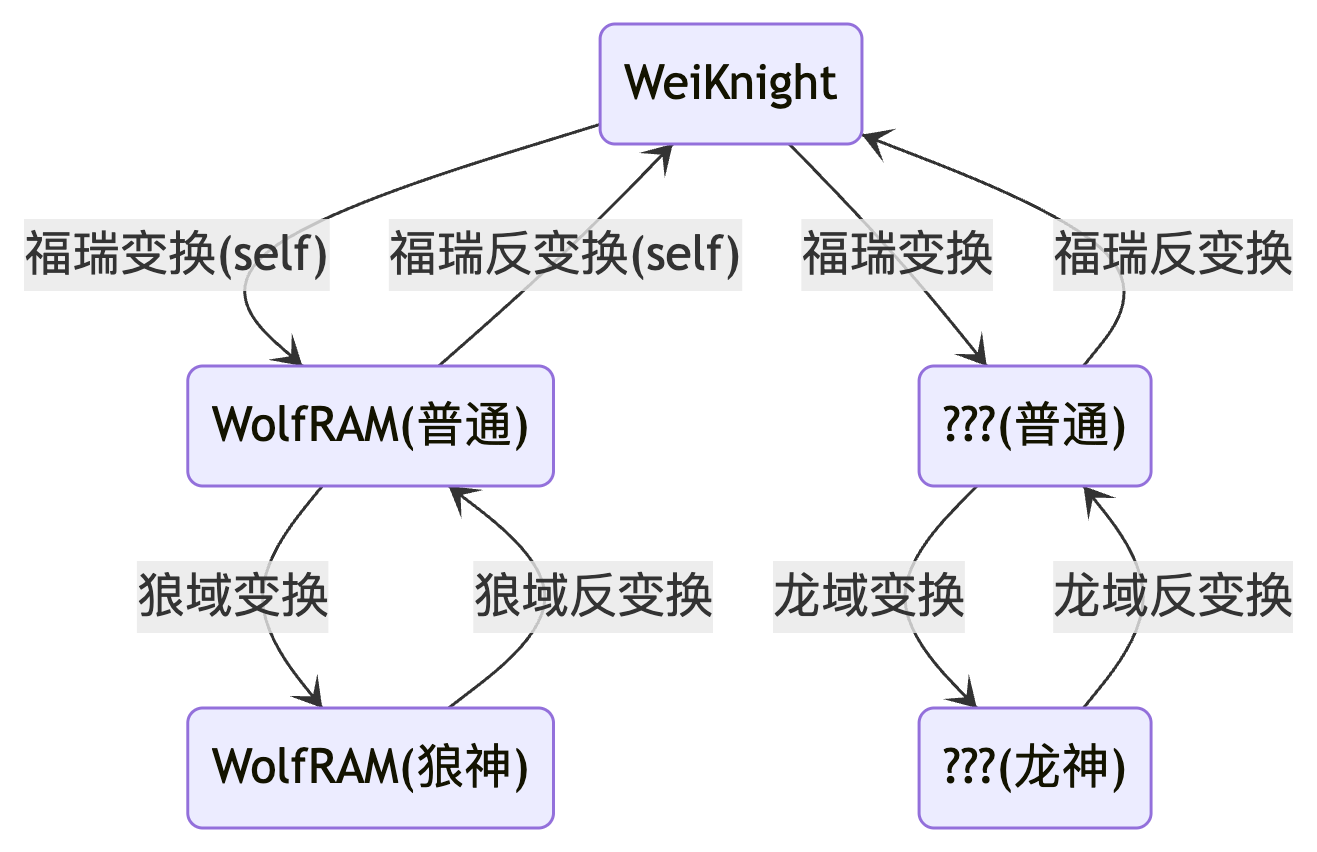
\includegraphics[width=0.6\textwidth]{figure/transform.png}
    \caption{三者变换关系}
    \label{fig:transform}
\end{figure}

其中self表示是自设变换。意味着\wf{}和\wkn{}具有同样的意识,
而成为\dr{}的福瑞变换更类似在\dr{}的身体里添加了新的意识,但无法控制\dr{}的身体;
\dr{}本身有自己的意识。

这些变换是基于世界的变换,即变换需要进入其他的世界。

此外\wf{}和\dr{}设定上是好友,偶然的机会他们在M2世界的酒吧相遇,发现二者经历相似,遂成为好友(很好的那种)。

\chapter{\wkn{}的OC的介绍}

本章主要介绍\wkn{}的OC。根据世界观,\wkn{}的OC主要包括\wf{}和\dr{}。
\begin{introduction}
    \item \wf{}
    \item \dr{}
\end{introduction}

\section{\wf{}}

\subsection{普通形态}
\noindent
\begin{figure}[H]
    \begin{minipage}[c]{0.48\textwidth}
        \centering
        
\includegraphics[width=\linewidth]{wolfram/normal.png} % 普通形态立绘路径
        \caption{\wf{} 普通形态立绘\\\centering 画师@Boiledhalf}
        \label{fig:wfnormal}
    \end{minipage}
    \hfill
    \begin{minipage}[c]{0.48\textwidth}
        \textbf{状态来源:} 处于\textbf{非}狼界WF时保持 \\
        \textbf{表现特征:}
        \begin{itemize}
            \setlength\itemsep{0em}
            \item 蓝色狼兽人
            \item 左侧脸上有一道闪电纹路
            \item 穿着黑色科技风外套
        \end{itemize}
        \textbf{行为习惯:} 喜逻辑推理与公式建模,偶尔模仿狼嚎 \\
        \textbf{人格特质:} 冷静、高智、效率优先,社交理性,但不排斥交往\\
        \textbf{日常职业:} 主职业为程序员,偶尔有雇佣兵的任务。\\
        \vspace*{\fill}
    \end{minipage}
\end{figure}

\newpage

\subsection{狼神形态——雷之狼神}

\noindent
\begin{figure}[H]
    \begin{minipage}[c]{0.48\textwidth}
        \centering
        
\includegraphics[width=\linewidth]{wolfram/god.png} % 狼神立绘路径
        % \vspace{0.5em}
        \centering
        \caption{\wf{} 狼神形态立绘\\ \centering 画师还没画(得等个2年)}
        \label{fig:wfgod}
    \end{minipage}
    \hfill
    \begin{minipage}[c]{0.48\textwidth}
        \textbf{状态来源:} 当位于自己掌控的世界(狼界WF)内时自动切换 \\
        \textbf{表现特征:}
        大部分与普通形态保持一致。不同点:
        \begin{itemize}
            \setlength\itemsep{0em}
            \item 额头上有特殊标志
            \item 右眼颜色变为红色
            \item 双手手背浮现出闪电的标志
            \item 双眼常亮电弧
        \end{itemize}
        \textbf{装备变化:} 身披狼神战袍 \\
        \textbf{性格特征:} 性格与通常形态基本一致,但神性更强,充满威压感\\
        \vspace*{\fill}
    \end{minipage}
\end{figure}

\newpage

\subsection{\wf{}的能力介绍}
\subsubsection{基础能力:矢量控制}
\textbf{矢量控制}是操纵特定类型矢量的基础能力,
视觉表现为蓝色半透明箭头轮廓,
\wf{}可以对选定矢量进行以下操作:

\begin{itemize}
    \item \textbf{矢量添加}:在物体上直接添加一个矢量,矢量的大小有某个最大限制
    \item \textbf{矢量删除}:使特定矢量归零,例如消除冲击力或抵消电磁场
    \item \textbf{大小调节}:按比例缩放矢量模长,矢量的大小有某个最大限制
    \item \textbf{方向操控}:改变矢量指向,产生旋转效果,最大的旋转角度有某个最大限制
\end{itemize}

适用矢量类型较为有限。只能操控以下种类的矢量:
\begin{itemize}
    \item 力学矢量:力($\bm{F}$)、速度($\bm{v}$)、加速度($\bm{a}$)
    \item 场效应矢量:电场强度($\bm{E}$)、磁感应强度($\bm{B}$)
    \item 以上矢量的衍生矢量:即以上矢量通过加法、数乘、叉乘运算后得到的矢量
\end{itemize}

\subsubsection{狼神能力:雷霆掌控}

\textbf{雷霆掌控}是操纵雷电元素的能力,
身为雷之狼神的\wf{}拥有下列雷元素的能力:

\begin{itemize}
    \setlength\itemsep{0em}
    \item \textbf{雷电生成}:从体内或大气中产生高压雷电
    \item \textbf{形态操控}:将雷电塑造成剑等战斗用攻击形态
    \item \textbf{精准打击}:控制闪电劈落的位置
    \item \textbf{雷电吸收}:免疫雷击伤害并转化为自身能量
    \item \textbf{风暴召唤}:引发一定半径的雷暴天气
    \item \textbf{闪电疾行}:一定距离内电流化瞬移
\end{itemize}

\newpage

\section{\dr{}}
\subsection{普通形态}
\begin{figure}[H]
    \begin{minipage}[c]{0.48\textwidth}
        \centering
        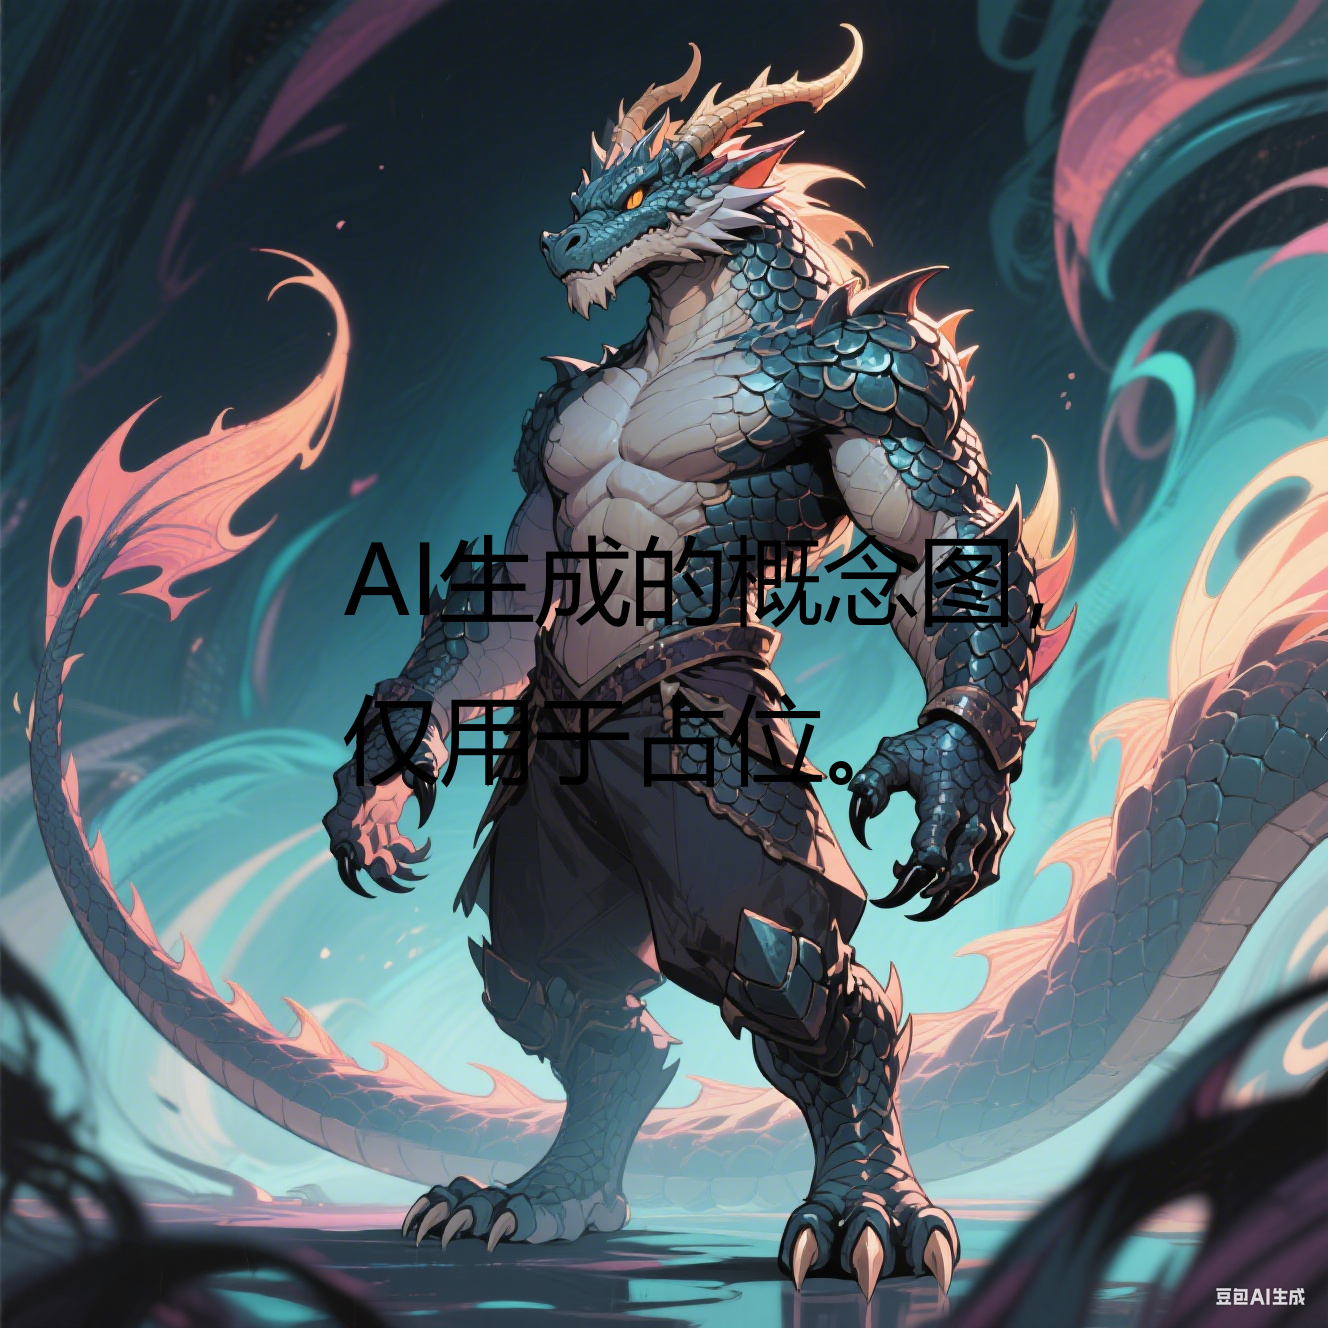
\includegraphics[width=\linewidth]{drago/normal.png}
        \caption{\dr{} 普通形态立绘\\\centering 画师待指定}
        \label{fig:drnormal}
    \end{minipage}
    \hfill
    \begin{minipage}[c]{0.48\textwidth}
        \textbf{状态来源:} 处于\textbf{非}龙界DR时保持\\
        \textbf{表现特征:}
        \begin{itemize}
            \setlength\itemsep{0em}
            \item 红色龙兽人
            \item 眼睛为紫色
            \item 无实体翅膀
            \item 戴着半框眼镜
            \item 双侧眼角有烈焰纹路
        \end{itemize}
        \textbf{行为习惯:} 喜欢打音游,同时还热爱音乐,时不时中二病发作哼歌。\\
        \textbf{人格特质:} 热情洋溢、善于调动气氛,享受与人互动,教学时充满表演欲\\
        \textbf{日常职业:} 某学院特聘术士教师,周末有时在Livehouse演奏\\
        \vspace*{\fill}
    \end{minipage}
\end{figure}

\newpage

\subsection{龙神形态——炎之龙神}

\noindent
\begin{figure}[H]
    \begin{minipage}[c]{0.48\textwidth}
        \centering
        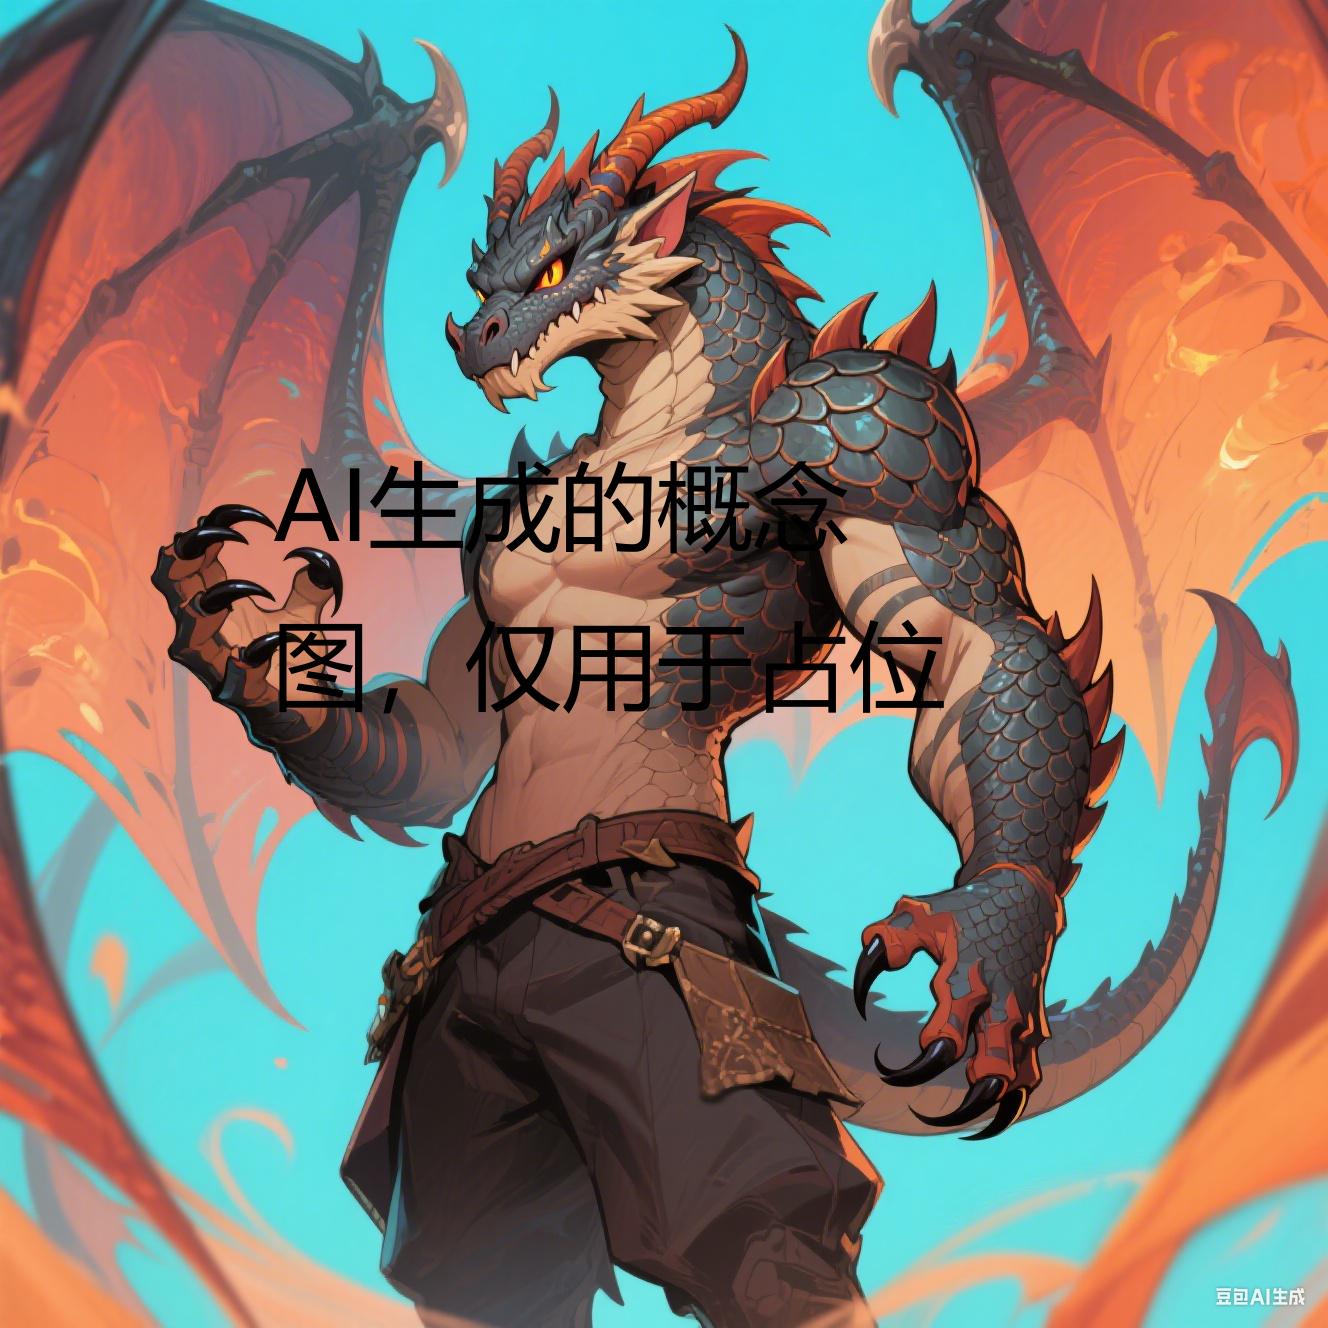
\includegraphics[width=\linewidth]{drago/god.png}
        \caption{\dr{} 龙神形态立绘\\ \centering 画师待指定}
        \label{fig:drgod}
    \end{minipage}
    \hfill
    \begin{minipage}[c]{0.48\textwidth}
        \textbf{状态来源:} 当位于自己掌控的世界(龙界DR)时自动切换\\
        \textbf{表现特征:}
        基础特征与普通形态相同,差异点:
        \begin{itemize}
            \setlength\itemsep{0em}
            \item 瞳孔转为熔金色
            \item 能够幻化出火焰的翅膀
            \item 眉心出现火形印记
            \item 尾尖出现燃烧的火焰
        \end{itemize}
        \textbf{装备变化:} 身披龙神战袍\\
        \textbf{性格特征:} 与普通形态性格类似,但增添神性威严,火焰会随情绪剧烈波动\\
        \vspace*{\fill}
    \end{minipage}
\end{figure}

\newpage

\subsection{\dr{}的能力介绍}
\subsubsection{基础能力:节奏幻奏}
\begin{itemize}
    \item 召唤虚拟音游键盘攻击,伤害由节奏判定精度决定
          \begin{itemize}
              \item \textcolor{yellow!75!black}{\textbf{PERFECT+}}:暴击(\texttimes 150\%~200\%)
              \item \textcolor{teal}{\textbf{PERFECT}}: 普通伤害(\texttimes 100\%)
              \item \textcolor{blue}{\textbf{GOOD}}: 普通伤害(\texttimes 80\%)
              \item \textcolor{red}{\textbf{MISS}}: 无伤害(连击归零)
          \end{itemize}
    \item 大P的判定范围为\(\pm 25 \text{ms}\),小P判定范围为\(\pm 50 \text{ms}\),GOOD判定范围为\(\pm 80 \text{ms}\)。
    \item \textbf{Combo加成}: 连击加成:每10连击提升5\%伤害(上限30\%)
\end{itemize}

\subsubsection{龙神能力:炎龙神焰}

\textbf{炎龙神焰}是操纵火焰元素的能力,
身为炎之龙神的\dr{}拥有下列火元素的能力:

\begin{itemize}
    \setlength\itemsep{0em}
    \item \textbf{神焰生成}:直接产生高温烈焰
    \item \textbf{形态操控}:将火焰塑造成各种形态,如火球
    \item \textbf{温度掌控}:自由调节火焰温度
    \item \textbf{火焰吸收}:免疫火焰伤害并转化为自身能量
    \item \textbf{炼狱领域}:创造一定半径的绝对燃烧领域
    \item \textbf{炎龙之息}:喷射出高温的火焰
\end{itemize}

\chapter{Q\&A}
\section{Q\&A}


\chapter*{后记}






\end{document}
